
\begin{figure}
\begin{table}
\begin{tabular}{cc}
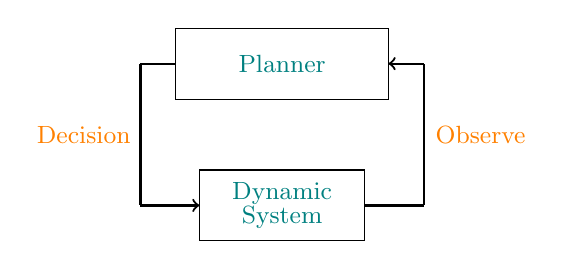
\begin{tikzpicture}[scale=0.6,font=\small,axis/.style={very thick, ->, >=sorangeth'}]

\draw [black=100](-2.25,-1.25) rectangle (2.25,0.25);
\node[teal] at(0,-0.5) {Planner};
%\node[black] at(0,-0.75) {};

\draw [black=100](-1.75,-4.25) rectangle (1.75,-2.75);
\node[teal] at(0,-3.25) {Dynamic};
\node[teal] at(0,-3.75) {System};

\node[orange] at(4.2,-2){\color{orange}{Observe}};


\node[orange] at(-4.2,-2){Decision};

\draw[thick,-](-2.25,-0.5)--(-3,-0.5);
\draw[thick,-](-3,-0.5)--(-3,-3.5);
\draw[thick,->](-3,-3.5)--(-1.75,-3.5);

\draw[thick,->](3,-0.5)--(2.25,-0.5);
\draw[thick,-](3,-3.5)--(3,-0.5);
\draw[thick,-](1.75,-3.5)--(3,-3.5);

\end{tikzpicture}
&
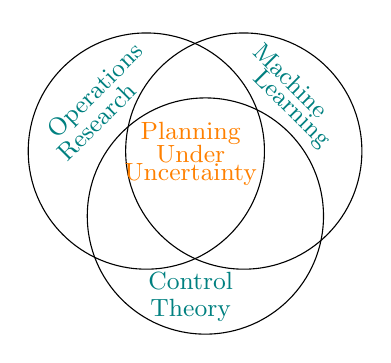
\begin{tikzpicture}[scale=0.75,font=\small,axis/.style={very thick, ->}]
\draw [] (0.9,0.5) circle (2);
\draw [] (-0.75,0.5) circle (2);
\draw [] (.25,-0.6) circle (2);
%\draw [] (-0.5,0.5) circle (2);
%\draw [] (0.5,-0.5) circle (2);
%\draw [] (-0.5,-0.5) circle (2);

\node[orange] at(0,0.8){Planning};

\node[orange] at(0,0.45){Under};
\node[orange] at(0,0.1){Uncertainty};

\node[teal,rotate=-45] at(1.7,1.7){Machine};
\node[teal,rotate=-45] at(1.7,1.2){Learning};

\node[teal,rotate=45] at(-1.6,1.5){Operations};
\node[teal,rotate=45] at(-1.6,1.0){Research};

\node[teal] at(-0,-1.7){Control};
\node[teal] at(-0,-2.2){Theory};
\end{tikzpicture}

\end{tabular}

\end{table}
%\caption*{No Explicit Labels; Control via Feedback }
\end{figure}
